\chapter{Raman Optical System}\label{chap:raman_optics}

\section{Chapter Outline}
This chapter presents in detail the optical system used to produce a
large collimated beam for driving Raman transitions. It begins with a
motivation of the need to minimise intensity gradients and wavefront distortions 
in~\SectionRef{sec:wavefront_req}. This is followed by a description
of the components that form the collimator
in~\SectionRef{sec:setup_ramanoptics}.
\SectionRef{subsec:setup_ramanmirror} presents an overview of the
retro-reflection assembly.
\section{Requirements}\label{sec:wavefront_req}
This section
outlines the optical characteristics of the light which affect the
sensitivity of the atom interferometer. These are discussed in the
context of this experiment, where gravity induces transverse motion
across the light. The light beams that drive the Raman transition have
a intensity profile that varies radially, e.g. along the axis parallel
to gravity. The motion of the atoms through
a gradient of intensity leads to a variation in the Rabi frequency that reduces the interferometer fringe
contrast and decreases acceleration sensitivity~\cite{Kim2017}.
This places requirements on the beam waist size, which are discussed
in~\SectionRef{subsec:fringe_beam_size}. 
\par\noindent
The atom interferometer senses acceleration through the second
derivative of the phase of the beat note between the two
counter-propagating light fields that drive the Raman transition. Any
such phase derivative that does not result from the acceleration of the atoms along
the Raman axis is a source of error.
One such source is distortion of the Raman beams wavefronts, which can
arise from transmission through rough optical elements.
%This is particularly apparent in
%the wavefront of the light. Optical distortions of the two Raman beams
%leads to an additional position-dependent phase shift. When there is
%significant transverse motion across the wavefront, this phase is not
%the same at each pulse and is not cancelled in the interferometer phase
%$\Delta \Phi$\footnote{Since $\Delta \Phi = \phi_1 - 2\phi_2 +
%\phi_3$, any effect which leads to a constant or linear phase shift at
%each pulse is not measured by the interferometer.}.  
In fact, the typical flatness of optical viewports is greater than
desired for making a sensitive accelerometer. To avoid the need for
optical viewports, the Raman optical system, described
in~\SectionRef{sec:setup_ramanoptics}, was mounted inside the
chamber and built using optical elements that were manufactured to
far better surface
qualities than conventional optics. 
The effect of wavefront distortions as a source of phase noise is
discussed in~\SectionRef{subsec:fringe_wavefront}.
\subsection{Gradients of Intensity}\label{subsec:fringe_beam_size}
The effects of a gradient of intensity on the fringe contrast can be shown by
considering an ensemble of atoms with a Gaussian
distribution of position. Neglecting the effect of the ensemble's velocity distribution on
the Raman detuning, the Rabi frequency \(\Omega\)
varies only as a function of the radial displacement $\rho$ from the optic axis. The
fringe contrast is then a convolution of the contrast for a
single atom with the atomic density distribution
\begin{equation}
	\mathcal{C} = \int_0^\infty
  \frac{\rho}{\sigma_c^2}e^{-\rho^2/(2\sigma_c^2)}
  c\left(\Omega(\rho-\rho_1),\Omega_(\rho-\rho_2),\Omega(\rho-\rho_3)\right)
  \;\mathrm{d}\rho
	\label{eq:cloud_contrast}
\end{equation}
where \(\sigma_c\) is the rms radius of the atom cloud projected along any one
Cartesian axis. 
The fringe contrast for a single atom, denoted by $c$, is
defined in \EquationRef{eq:fringe_contrast}. The arguments refer to
the Rabi frequency during each pulse. The duration of each pulse is
chosen such that an atom at the centre-of-mass radius $\rho_i$ has a $\pi/2$ or $\pi$
rotation. It is
assumed that the two light beams which drive the Raman transition have the same
waist size and Rabi frequency, determined by the product of the
electric fields (see~\EquationRef{eq:rabi_freq}). Therefore, the
position-dependent Rabi frequency is
\begin{equation}
	\Omega(r) = \Omega_0 e^{-2 \rho^2/w^2}
\end{equation}
where \(\Omega_0\) is the Rabi frequency along the optic axis and \(w\) is the
waist size -- the distance at which the electric field falls to \(1/e\) of its
peak value. 
\par\noindent
\FigureRef{fig:raman_fringecontrast} shows the fringe contrast as a function as beam waist for an atom cloud of
rms radius \(\sigma_c = \sivalue{5}{\milli\metre}\) and a time between
interferometer pulses of \(T = \sivalue{25}{\milli\second}\) for three
cases. The blue curve shows the contrast when the atom cloud is initially at the
centre of the laser and falls from rest under gravity so that centre-of-mass coordinates are
\(\left(0, -\frac{1}{2}g T^2, -2 g T^2\right)\) respectively. The
orange curve includes the vertical velocity of
$u =$ \sivalue{25}{\cm\per\s} that the atoms are launched with by the
molasses. Finally, the green curve displaces the starting position of
the atom cloud to an initial position $\rho_0 = \frac{u T}{2} - \frac{g
T^2}{4}$, so that each pulse is displaced by the same amount from the
centre of the beam and the cloud sees the same intensity gradient. For small beam waists, the intensity
gradient across the cloud significantly reduces the fringe contrast,
particularly when the atoms are not launched. A beam waist much greater than the width of the cloud is necessary to achieve a
large contrast. 
\begin{figure}[!htbp]
	\centering
	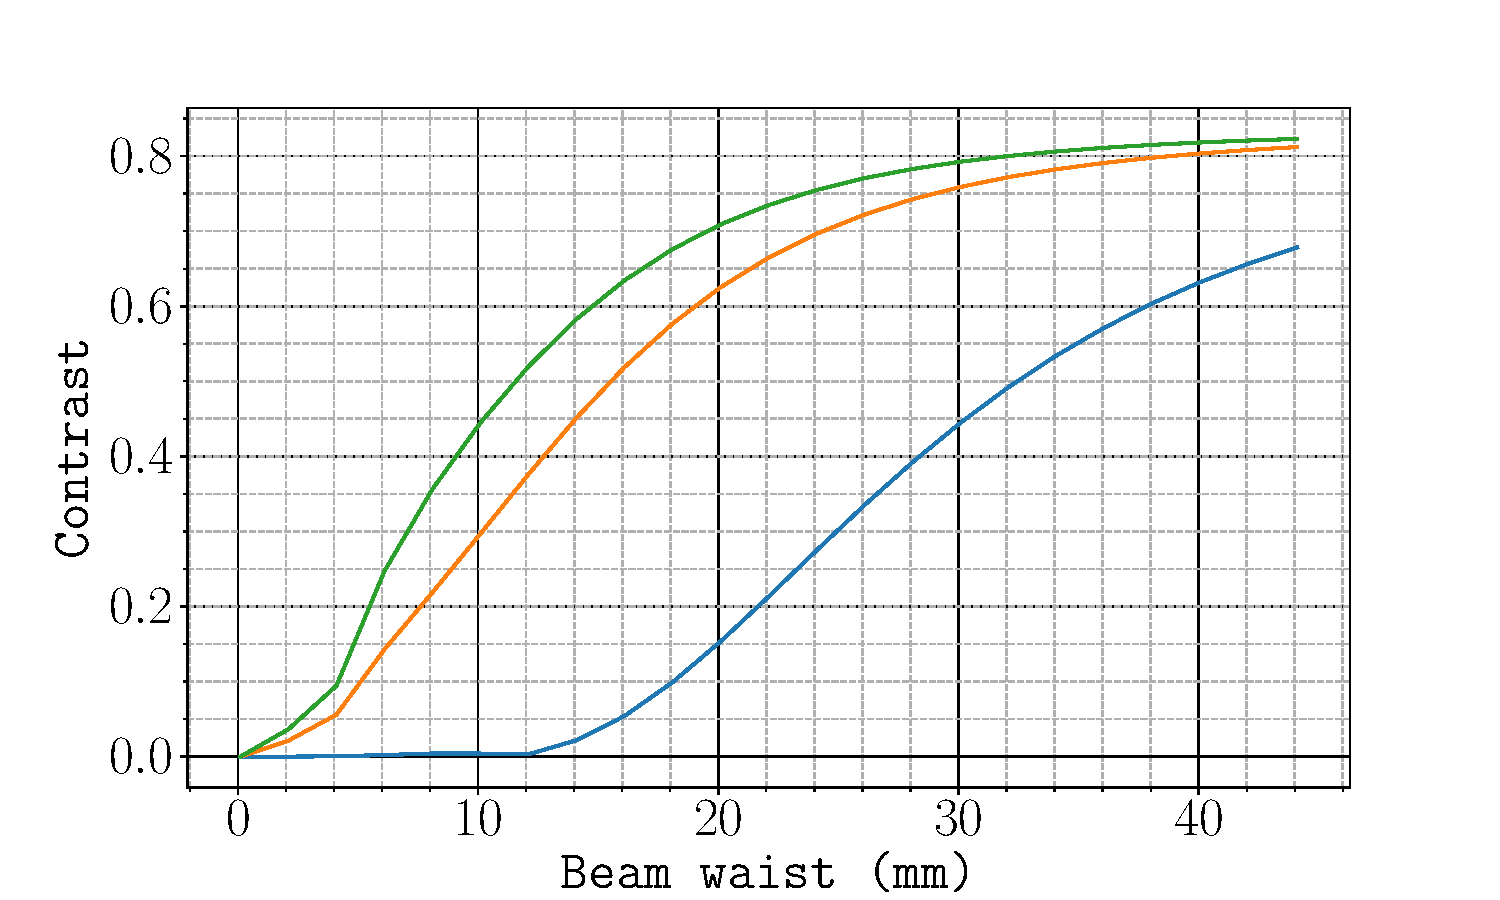
\includegraphics[width=0.7\textwidth]{fringe_contrast.pdf}
	\caption[Simulated fringe contrast vs beam waist size]{Simulated fringe
		contrast as a function of waist size \(w\) for an atom cloud falling under
		gravity. This model assumes a Gaussian distributed atomic density
    with a rms radius \(\sigma_c = \sivalue{5}{\milli\metre}\) and a time between
		interferometer pulses of \(T = \sivalue{25}{\milli\second}\). The
    blue curve shows the contrast when the atoms fall from rest under gravity.
    The orange curve includes the vertical launch velocity provided
    during the molasses phase. In the green curve, the atoms are
    displaced from the centre such that each pulse has the same
  intensity gradient (see text).} 
  %For smaller
	%	beam waists the subsequent interferometer pulses have a larger intensity
	%	gradient across the atom ensemble, which increases the dephasing of the two
	%	states and reduces the interferometer fringe contrast.}
	\label{fig:raman_fringecontrast}
\end{figure}
\par\noindent
The velocity distribution of the atoms introduces a detuning to each
interferometer pulse due to the Doppler shift, as well as modifying
the spatial distribution due to thermal expansion.
\FigureRef{fig:phase_vel} shows the fringe contrast when including the
one-dimensional velocity distribution of an atom ensemble with a
temperature of \sivalue{5}{\micro\K}. The most significant difference is
for small beam waists in
the case of no initial launch velocity, where the contrast is now less
suppressed. Aside from this, the fringe contrast is not hugely
affected by the velocity distribution of the atoms. 
\begin{figure}[htpb]
  \centering
  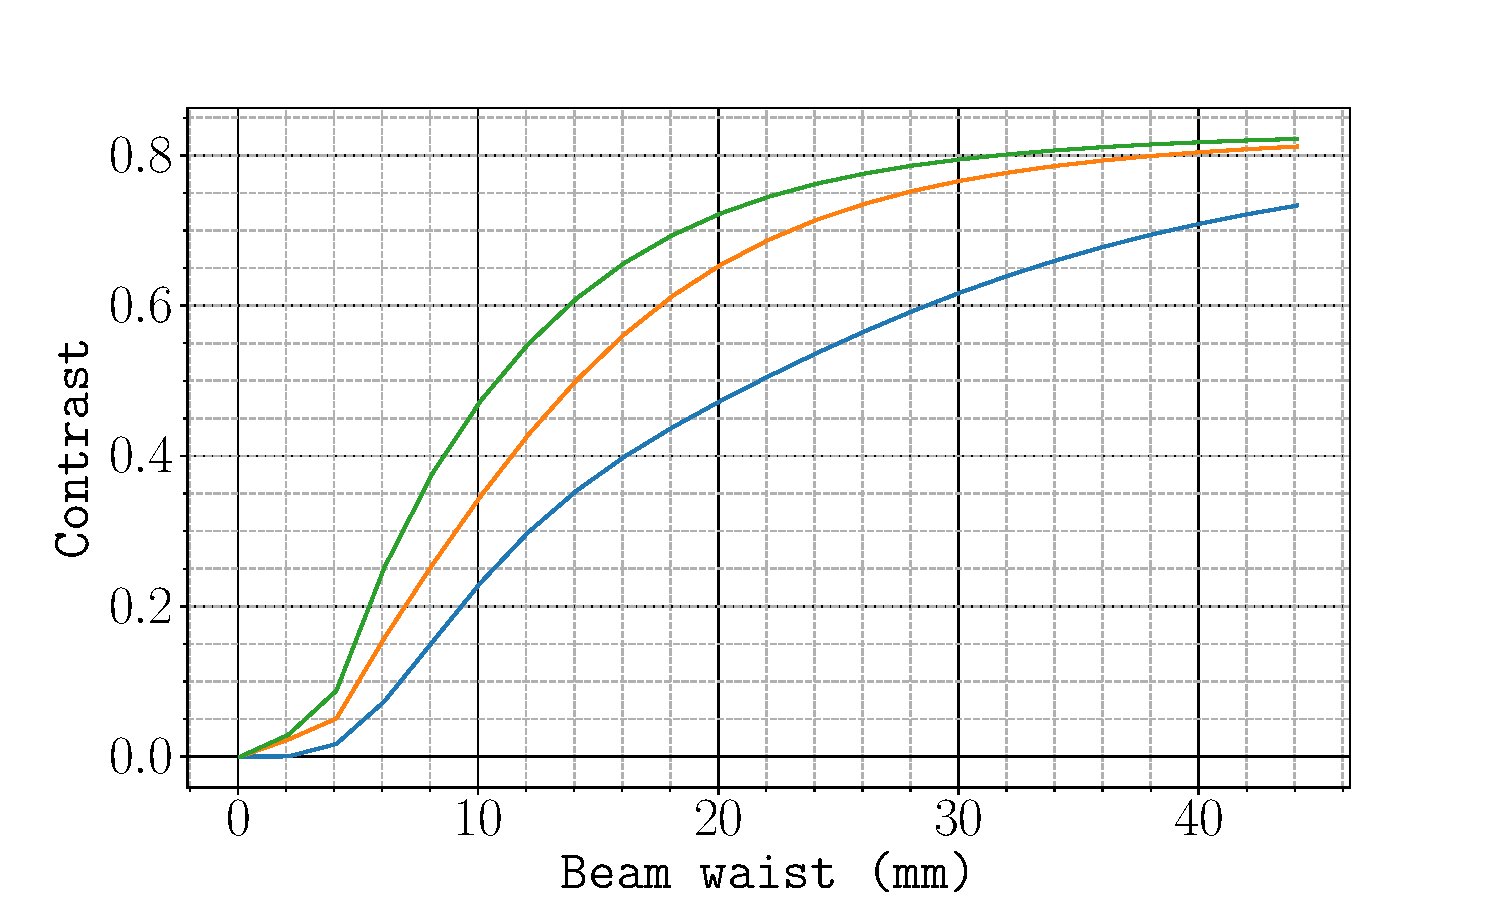
\includegraphics[width=0.7\linewidth]{fringe_contrast_vel.pdf}
  \caption[Simulated fringe contrast vs beam waist size including a
  thermal velocity distribution.]{Simulated fringe contrast as a function of waist size $w$,
  including the effects of a velocity distribution along the Raman
beam corresponding to a temperature of \sivalue{5}{\micro\K}. The other
parameters are the same as those used
in~\FigureRef{fig:raman_fringecontrast}.}
  \label{fig:phase_vel}
\end{figure}
\subsection{Wavefront Distortions}\label{subsec:fringe_wavefront}
\subsubsection{Systematic Effects}
The field that drives the Raman transition comes from the
superposition of the two counter-propagating Raman beams. The optical
system used to collimate the Raman beams is presented below,
in~\SectionRef{sec:setup_ramanoptics}. Ideally,
the Raman beams are Gaussian beams and with a beam
waist of \sivalue{35}{\mm}, the Rayleigh length $z_R \approx
$ \sivalue{5}{\km} means that when collimated, the two beams have an
almost identical radius of curvature. In this case, the effective field will have a planar wavefront.
However, if the beams are not collimated they will have different
radii of curvature and their superposition will therefore
have a parabolic wavefront. Each Raman pulse will impress a different
phase to an atom falling under gravity, leading to a component of the
interferometer phase that does not cancel out.
\FigureRef{fig:collimation_wavefront} shows the effects of poor
collimation on the effective Raman wavefront for increasing divergence
angles, where it can be seen that the curvature of the Raman wavefront
similarly increases. \FigureRef{fig:collimation_interferometer} shows yhe corresponding interferometer phase for an
atom falling from rest under gravity with a pulse separation of $T=$
\sivalue{25}{\ms}. A divergence angle of
\sivalue{1}{\milli\radian} results in an interferometer phase
contribution of \sivalue{8e-7}{\radian}.  
Provided that the beams are reasonably
well-collimated, this effect can be largely neglected as it is
unlikely to be a dominant source of error. 
%\begin{figure}[!htbp]
%	\centering
%	\def\svgwidth{\columnwidth}
%	\subfloat[][]{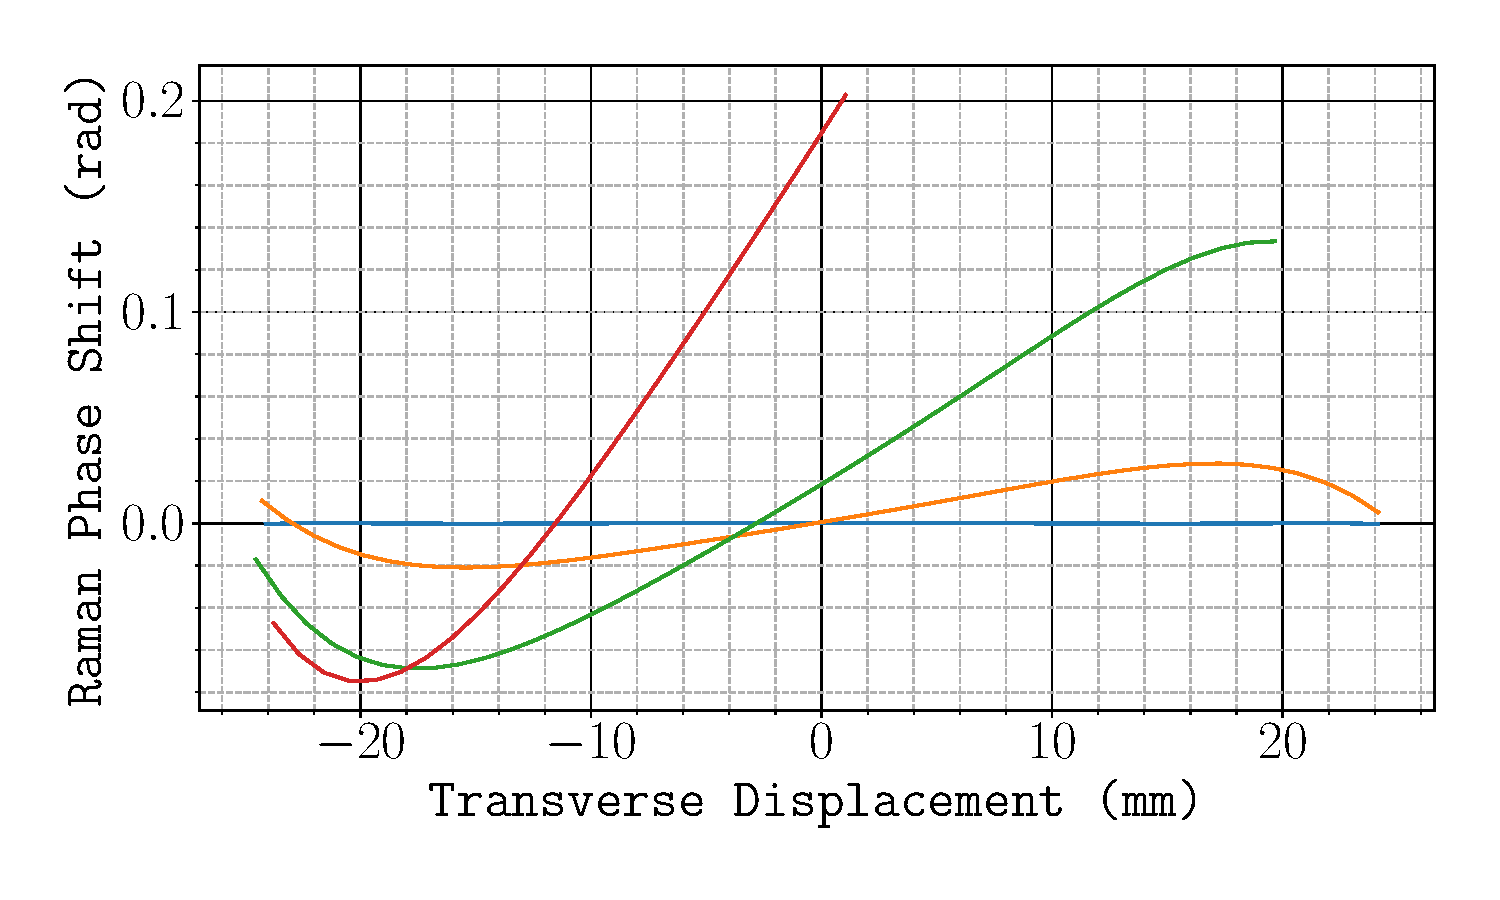
\includegraphics[width=0.4\textwidth]{wavefront_transverse.pdf}\label{fig:raman_wave_transverse}}
%	\subfloat[][]{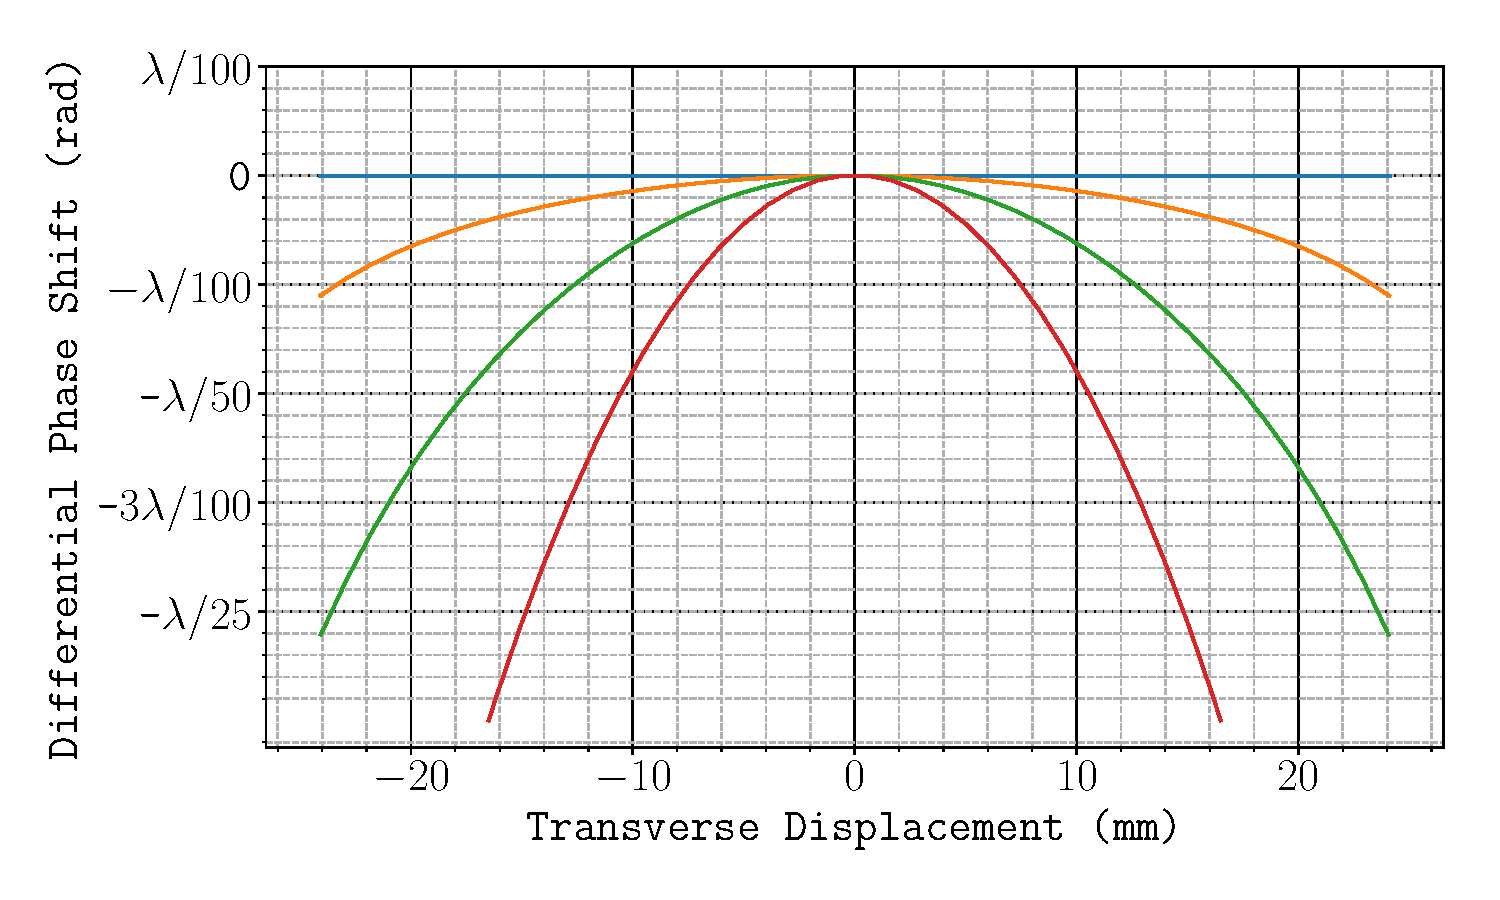
\includegraphics[width=0.4\textwidth]{wavefront_longitudinal.pdf}\label{fig:raman_wave_longitudinal}}
%	\caption[Simulated wavefront distortion for longitudinal and transverse fibre
%		misalignment]{Simulated wavefront distortion for longitudinal and transverse
%		fibre misalignment. Rays from a point source with a divergence angle
%		corresponding to a \ac{na} of 0.12 are propagated through the Raman optical
%		system. Rays corresponding to the reflected beam are propagated further with
%		the assumption that the mirror is perpendicular to the optic axis. The first
%		set of rays propagates \sivalue{43}{\milli\metre} and the second propagates
%		\sivalue{129}{\milli\metre}. The wavefront for each beam is calculated by
%		taking the slope of each ray and subtracting from the slope of the central
%		ray. The wavefront of the effective field that drives the Raman transition
%		is the difference of these two wavefronts. (a) shows the distortion of the
%		wavefront for a transverse misalignment of the fibre for a displacement of
%		\sivalue{0}{\milli\metre} (blue), \sivalue{0.5}{\milli\metre} (orange)
%		\sivalue{1}{\milli\metre} (green) and \sivalue{1.5}{\milli\metre}
%		(red) from
%		the front focal point. (b) shows the wavefront for longitudinal
%		displacements of \sivalue{0}{\milli\metre} (blue),
%		\sivalue{0.3}{\milli\metre} (orange)
%		\sivalue{0.6}{\milli\metre} (green) and \sivalue{1}{\milli\metre}
%		(red).}\label{fig:fig_label}
%\end{figure}
\begin{figure}[!htbp]
	\centering
	\def\svgwidth{\columnwidth}
	\subfloat[][]{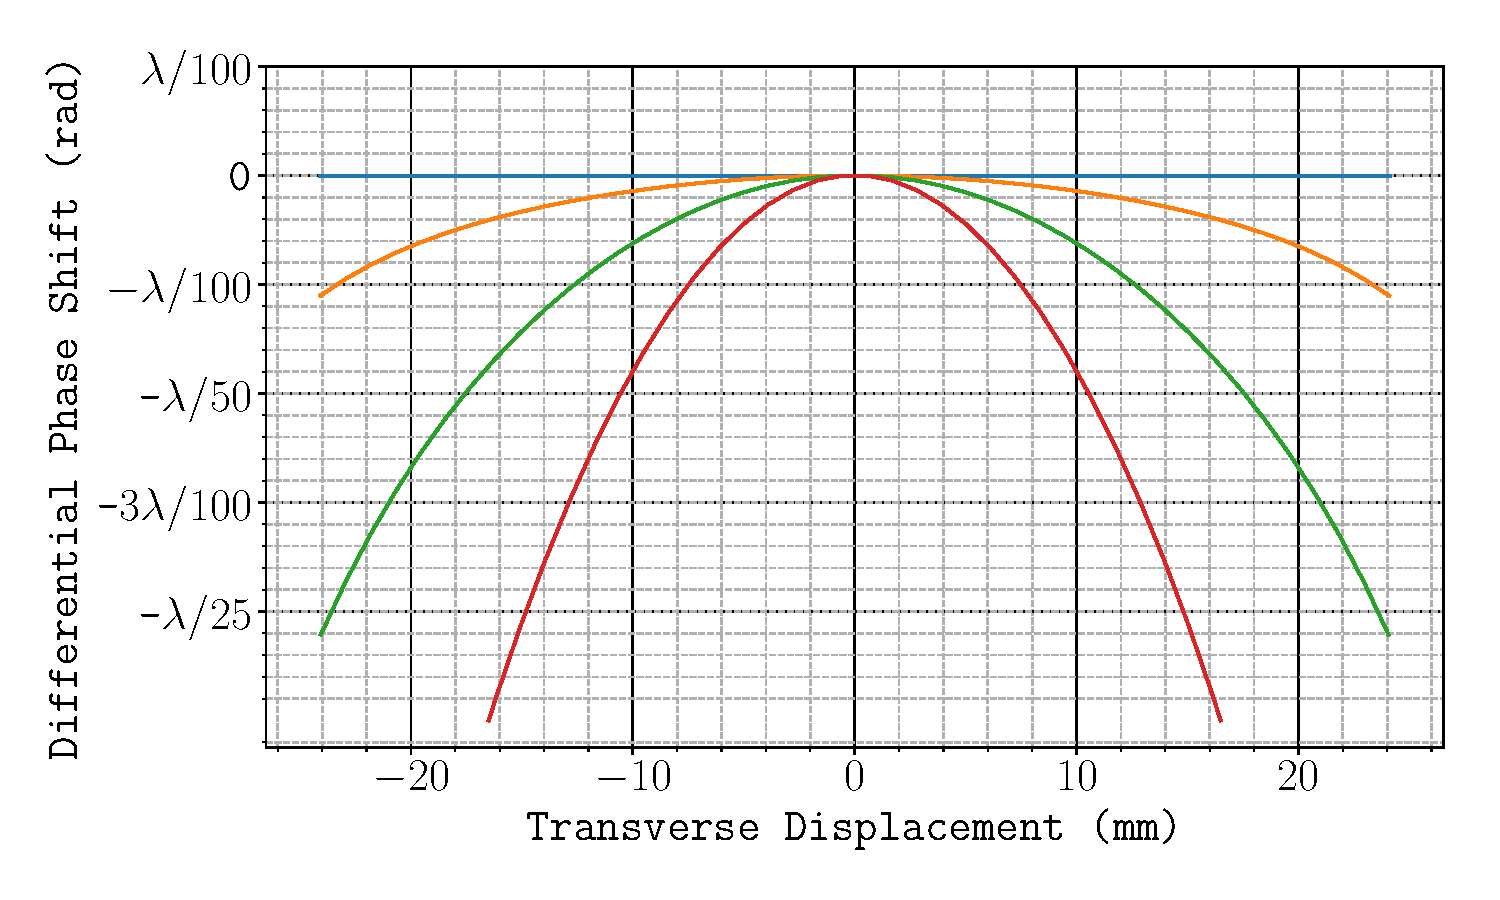
\includegraphics[width=0.4\textwidth]{wavefront_longitudinal.pdf}\label{fig:collimation_wavefront}}
	\subfloat[][]{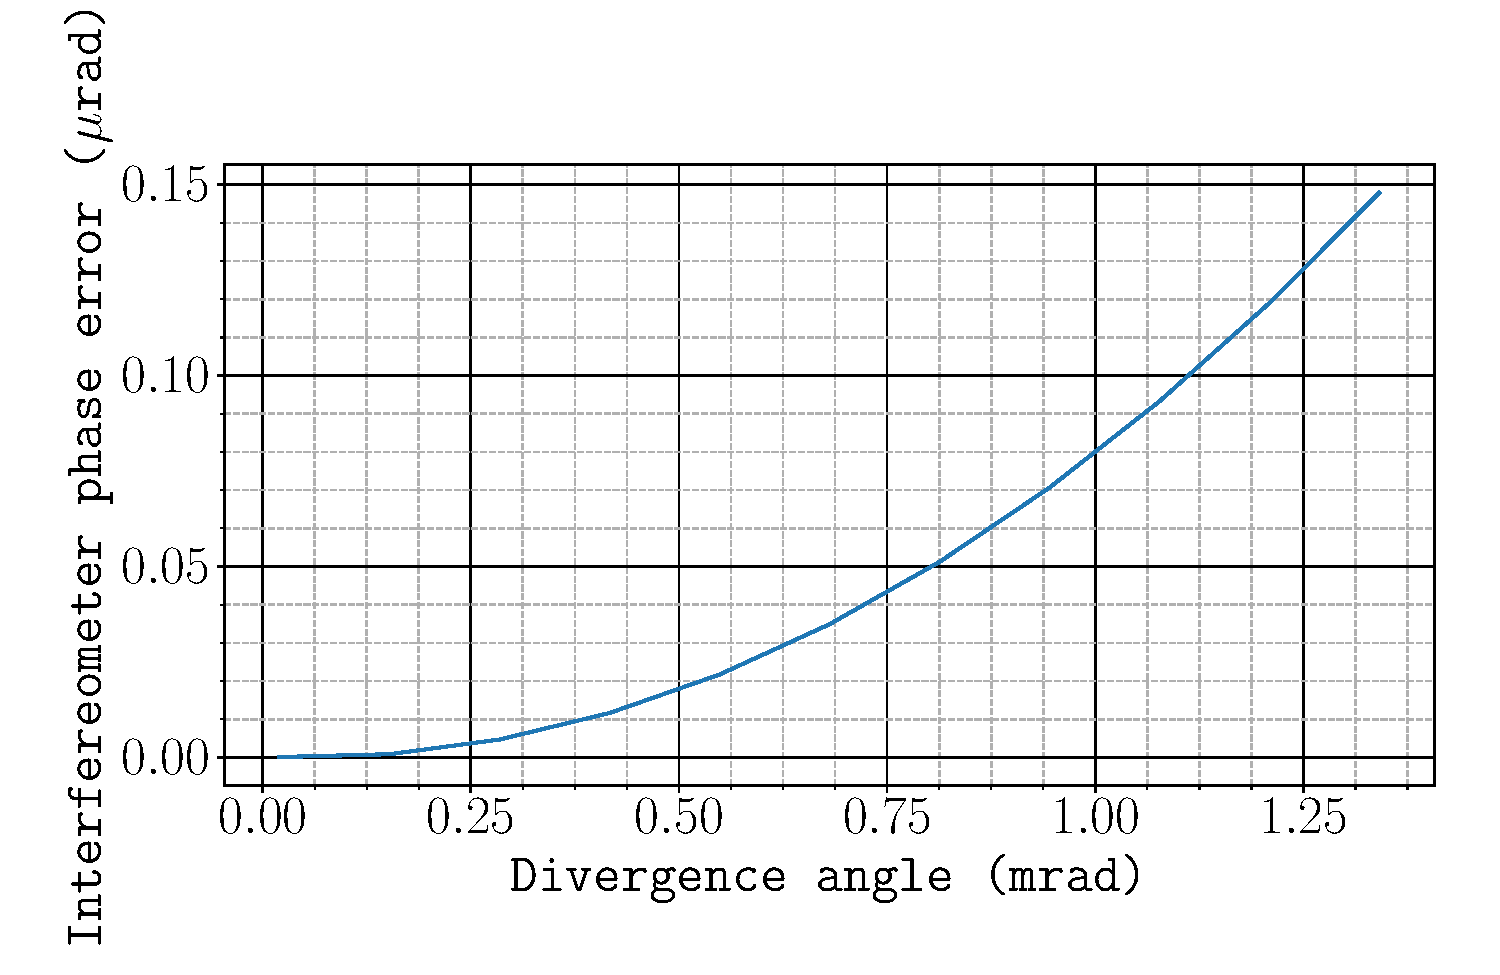
\includegraphics[width=0.4\textwidth]{collimation_phase_error.pdf}\label{fig:collimation_error}}
	\caption[Wavefront distortion and interferometer phase error for
  diverging Raman beams.]{Wavefront distortion and interferometer phase error for
  diverging Raman beams. The wavefront is calculated by propagating
  the two Raman beams. Rays corresponding to the reflected beam are propagated further with the assumption that the mirror is perpendicular to the optic axis. The first
		set of rays propagates \sivalue{43}{\milli\metre} and the second propagates
		\sivalue{129}{\milli\metre}. The wavefront for each beam is calculated by
		taking the slope of each ray and subtracting from the slope of the central
		ray. The wavefront of the effective field that drives the Raman transition
    is the difference of these two wavefronts. \textbf{(a)} shows the distortion of the
		wavefront for divergence angles of
		\sivalue{20}{\micro\radian} (blue), \sivalue{400}{\micro\radian} (orange)
		\sivalue{800}{\micro\radian} (green) and
    \sivalue{1.2}{\milli\radian} (red). \text{(b)} shows the resultant
    interferometer phase error as a function of divergence angle for an atom falling under gravity
    starting at rest on the optic axis.  
		}\label{fig:collimation_error_plots}
\end{figure}
\par\noindent
A more significant contribution 
arises if there is a tilt of the beams. \FigureRef{fig:perfect_retro}
presents the configuration when the incoming beam is tilted from the
optic axis, but is perfectly retro-reflected. The Raman wavefront is
planar, but the Raman axis is tilted from the optic axis. If the optic
axis is perpendicular to the axis of gravitational
acceleration, then the interferometer will measure a component of
gravitational acceleration $g \sin(\theta)$. If we require that this
acceleration error is no greater than \sivalue{100}{\nano\g}, then
this is equivalent to requiring that the tilt of the Raman axis is
less than \sivalue{0.1}{\micro\radian}. Such a tilt can be caused by a
displacement of the input fibre from the optic axis. This is discussed
in more detail in~\SectionRef{subsec:setup_ramancollimator}.
\begin{figure}[!htbp]
	\centering
  \fontsize{12pt}{12pt}
  \resizebox{0.5\textwidth}{!}{\input{Retro_Perfect.pdf_tex}}
	\caption[Tilted Raman beams with perfect retro-reflection.]{Tilted
  Raman beams with perfect retro-reflection. The Raman wavefront
propagates along the Raman axis, indicated by the dotted line. The
optic axis is perpendicular to gravity such that the interferometer is
sensitive to a component of gravitational acceleration given by
$\textbf{g} \sin(\theta)$.}\label{fig:perfect_retro}
\end{figure}
\par\noindent
If the mirror is parallel with the optic axis, it does not perfectly
retro-reflect the tilted incoming beam. At a given transverse
displacement, both the incoming and reflected beams have the same
phase shift, so it is cancelled in the Raman phase difference. 
\FigureRef{fig:imperfect_retro} illustrates the wavefronts in this
case. The Raman wavefront is still planar, but the wavevectors of the
two beams are not colinear. The Raman wavevector along the optic axis
($\hat{\textbf{x}}$)
is now $\keff' =
(k_1-k_2)\cos(\theta)\hat{\textbf{x}} \approx  \keff (1-\theta^2)$. This leads to an
interferometer phase error of $\keff\theta^2 a T^2$. For an
acceleration of \sivalue{0.3}{\g} and $T = $ \sivalue{25}{\ms}, a tilt
of $\theta = $ \sivalue{0.18}{\milli\radian} gives an interferometer
phase error of \sivalue{1}{\milli\radian}. \SectionRef{sec:in_situ} describes a method
used to ensure good alignment of the mirror, which
renders this error negligible.
\begin{figure}[htpb]
  \centering
  \fontsize{12pt}{12pt}
  \resizebox{0.5\textwidth}{!}{\input{Retro_Imperfect.pdf_tex}}
  \caption[Imperfect retro-reflection with a tilted incoming beam.
  ]{Imperfect retro-reflection with a tilted incoming beam.
  Here, the mirror is perpendicular to the optic axis so that the
Raman phase has a planar wavefront (indicated by the dotted line) that
travels along that axis. The tilt of the two beams means that their
wavevectors are not colinear and the Raman wavevector is $\keff' =
(k_1-k_2)\cos(\theta)\hat{\textbf{x}}$, where $\hat{\textbf{x}}$ is
the optic axis.}
  \label{fig:imperfect_retro}
\end{figure}
\subsubsection{Random Sources of Phase}
The propagation through rough optical elements distorts
the wavefronts and introduce a spatially varying component of the
Raman phase that is independent
of acceleration. If this phase is common to both beams then it does
not affect the atomic phase induced by the Raman
transition. It is necessary only to consider the difference in the phase of
the two light fields. If an atom's trajectory is parallel with the Raman axis,
then this phase difference is the same at each laser pulse and makes
no contribution to the interferometer phase for that atom. On the other hand, 
the Raman phase difference can change if the atom moves transverse to
the Raman axis and that contributes to the interferometer phase of the
atom. If that is the same for all atoms in the cloud then we are once
again describing the systematic error discussed immediately above. If
it differs for different atoms, then there is a loss of fringe
visibility that we estimate now.
\par\noindent 
For simplicity, let us assume that the interferometer phase has a
Gaussian distribution over the cloud with a standard deviation of \(\sigma_\Phi 
\). Denoting the random interferometer phase as \(\delta\phi\), the
fringe pattern for a single atom is
\begin{equation}
	F = \cos\left(\phi + \delta\phi\right)^2
\end{equation}
Following from this, the fringe pattern averaged over the cloud is
\begin{align}
  \langle F \rangle & = \frac{1}{\sqrt{2\pi}\sigma_\Phi}\int
  \cos(\phi+\delta \phi)^2 \; e^{-\delta\phi^2/2\sigma_\Phi^2} \; \mathrm{d}\delta\phi \\
                    &= \frac{1}{2}(1+e^{-2\sigma_{\Phi}^2}\cos(2\phi)) 
\end{align}
This give a fringe contrast of
\begin{equation}
    \mathcal{C} = e^{-2 \sigma_\Phi^2}
\end{equation}
\FigureRef{fig:raman_phasenoise} shows the fringe contrast as a
function of this random phase. Given the high quality of the optical
elements (see~\SectionRef{sec:setup_ramanoptics}), it seems unlikely
that the wavefront will wobble by more than $\lambda/50$ over a
transverse region of \sivalue{5}{\mm}. I therefore expect that
$\sigma_\Phi$ will not exceed \sivalue{100}{\milli\radian} and hence
the loss of contrast from this mechanism will not be large. However,
one can see that it is important to use optical components of high
quality and that the standard $\lambda/20$ is likely to produce
fringes of low contrast.
\begin{figure}[htbp]
	\centering
	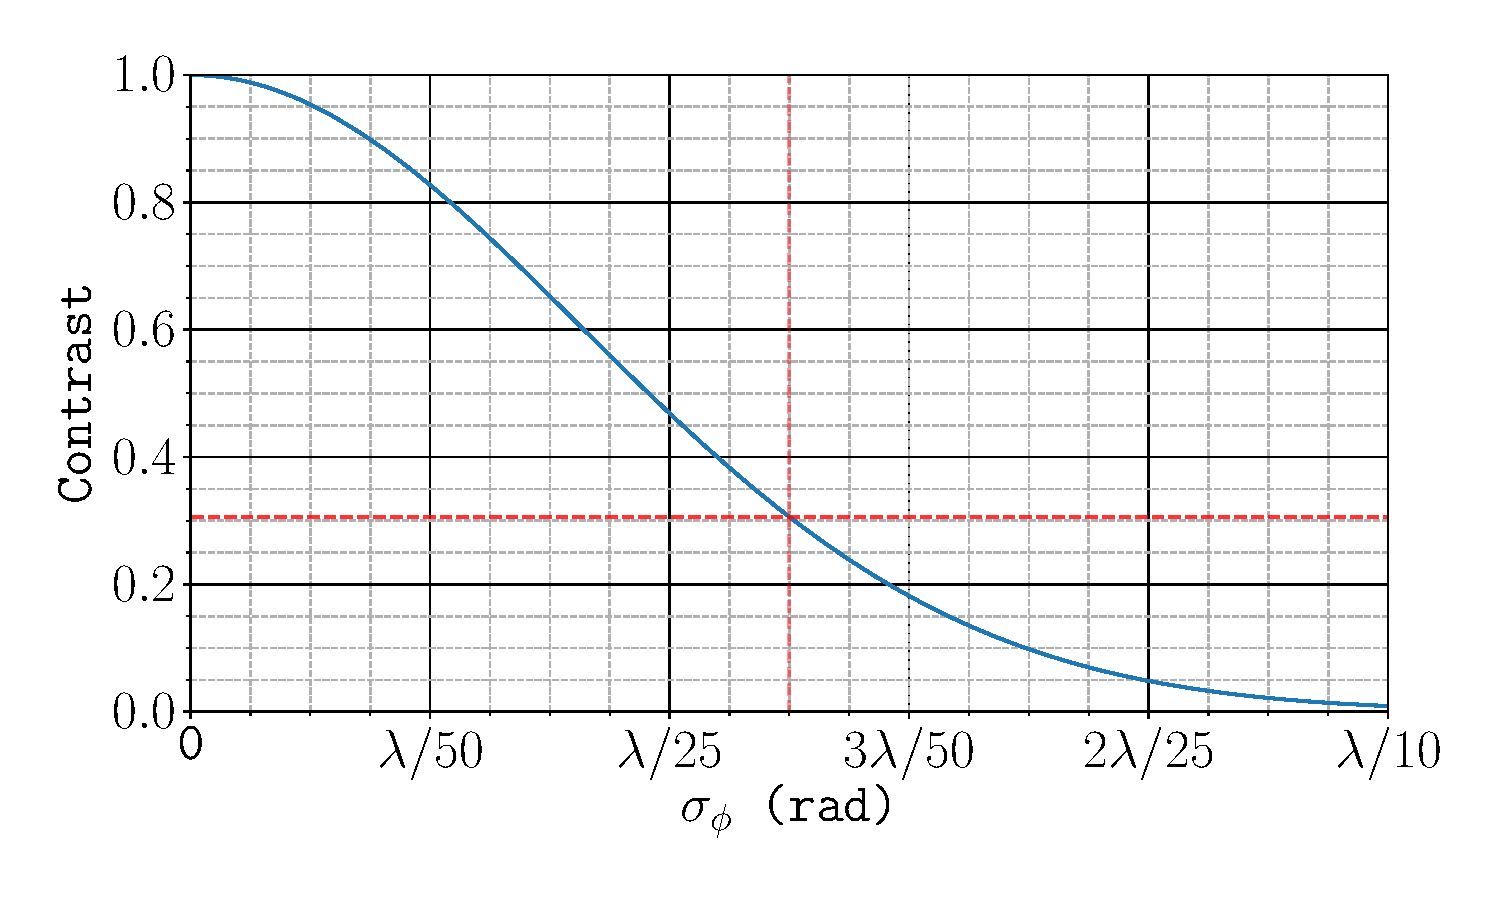
\includegraphics[width=0.7\textwidth]{phase_noise_contrast.pdf}
  \caption[Expected fringe contrast as a function of random phase
  contributions.]{Expected contrast as a function of random phase contributions. This
		assumes that the phase imprinted on an atom during each interferometer pulse
		has an additional random component that is Gaussian distributed around 0
		with a standard deviation of \(\sigma_\phi\). This random phase is also
		uncorrelated between each pulse so that the total can be obtained using
		Gaussian propagation of error. The dashed lines indicate the
    contrast for an rms phase uncertainty of \(\lambda/20\).}
	\label{fig:raman_phasenoise}
\end{figure}
\par\noindent
\section{Raman Optics}\label{sec:setup_ramanoptics}
The optical system used to produce the beams for driving Raman transitions,
will be referred to as the Raman Optics. For the reasons described in
the previous section, this was designed to
have good control over the flatness and orientation of the phase
fronts of the Raman beams. Principally, the entire
optical system was mounted inside the optical chamber so that the Raman light
does not pass through any optical viewports before interacting with the atoms.
This avoids the phase and polarisation distortions that are typically
introduced by passing light through a vacuum window.
\subsection{Component Overview}\label{subsec:setup_ramancollimator}
\begin{figure}[!htbp]
	\centering
	\def\svgwidth{\columnwidth}
  \fontsize{18pt}{18pt}
  \subfloat[][]{\raisebox{.4\height}{\scalebox{0.4}{\input{Figures/Chapter6/raman_optics.pdf_tex}\label{fig:raman_collimator}}}}\quad
	\subfloat[][]{\scalebox{0.4}{\input{Figures/Chapter6/mirror_mount.pdf_tex}\label{fig:mirror_mount}}}
	\caption[Drawings of the componets used in the Raman optics
		assemblies]{Diagrams of the components used in the Raman optical
      assemblies, not drawn to scale.
      \textbf{(a)} shows the collimator setup. Light is coupled into the chamber using a
		UHV fibre feedthrough. A pair of aspheric lenses is used to increase the
		divergence angle of the fibre output, before the light is collimated by a
		triplet lens. Finally, a quarter-wave plate is aligned so that it circularly
    polarises both collimated light fields. \textbf{(b)} illustrates the other half of the
		setup, which is used to retro-reflect the light. A second quarter-wave plate
		is used so that the reflected beams have the reversed circular
    polarisation. A MEMS accelerometer is mounted on the back of the
		mirror to measure vibrations. These components are all mounted on a
		piezo-controlled mirror mount whose tilt can be controlled from outside the
		vacuum chamber.}
	\label{fig:raman_optics}
\end{figure}
\FigureRef{fig:raman_collimator} presents a diagram of the components used to
send Raman light into the chamber and produce a collimated beam in the centre of
the chamber. The light is coupled into the chamber using a UHV compatible
\ac{pm} fibre, manufactured by Diamond photonics. This is a kapton-coated PM-780
HP fibre that is bonded on one end to a DN16 flange using an epoxy resin. The
external side of this flange has an FC/APC connector for coupling light from
another fibre. Inside the chamber, the output of the fibre plugs into to an FC/APC fibre
plate. This is clamped between a piece which bolts onto the inside of a DN63
flange and another stainless steel plate which bolts onto the rest of the optics
assembly. Fine adjustment of the position of the fibre along the optic axis is
achieved using shim plates with a thickness ranging from
200--\sivalue{300}{\micro\metre}. The fibre plate is free to rotate so that the
orientation of the fibre with respect to a \ac{qwp} at the output of the
collimator. This \ac{qwp} is manufactured by Light Machinery, and is described
further is \SectionRef{subsec:setup_ramanmirror}. When the fibre is correctly
orientated (e.g. when the slow axis of the fibre is at 45$^\circ$ to the slow
axis of the waveplate), the two Raman light fields are orthogonally circularly
polarised. \par\noindent The original design for the optical system consisted of
a triplet lens, as a system of three lenses is capable of correcting for the
five types of Seidel aberrations that distort rays of monochromatic light. This
was designed and manufactured by IC Optical Systems to deliver a
wavefront quality of $\lambda/100$. Another specification for
this lens system was that it had to produce a collimated beam with a waist size
of around \sivalue{35}{\milli\metre} so that the visibility of the
interferometer fringes would not be limited by the effects of intensity gradients across the
atoms. Unfortunately, the triplet was designed with an incorrect \ac{na}. With a
focal length of \sivalue{123.4}{\milli\metre} and a diameter of
\sivalue{50}{\milli\metre}, the triplet lens has a \ac{na} of 0.194. However,
the nominal \ac{na} for PM780-HP fibre used in the UHV compatible \ac{pm} fibre
is 0.12. Consequently, the light from this fibre did not fill the \ac{na} of the
triplet lens and produced a beam with a waist of \sivalue{13}{\mm}. 
%%{\huge Plot to illustrate this}. 
To address this issue, a pair of aspheric lenses was included to increase
the divergence angle of light from the fibre. These are manufactured by Thorlabs
and have a focal length of \sivalue{4.51}{\milli\metre} (352230-B) and
\(\sivalue{15.29}{\milli\metre}\) (352260-B), respectively, to give a
magnification of 3.39.
\subsection{Alignment and Collimation}
As one of the main motivations for mounting the Raman optics inside the vacuum
chamber was to reduce the effects of wavefront distortions, it is worth
highlighting how inaccurate alignment of the optics can lead to aberrations. As
previously discussed in \SectionRef{subsec:fringe_wavefront}, distortions of the
wavefront can produce a false acceleration and possible loss of
interferometer fringe visibility. 
Here, the same figures of merit as before are used to consider what misalignment
is acceptable to ensure that the false acceleration due to a distorted
wavefront is less than \sivalue{100}{\nano\g}.
%than \(\lambda/100\) after a transverse distance of
%\sivalue{12.5}{\milli\metre} (that being the distance fallen from rest
%after \sivalue{50}{\ms}. 
\par\noindent 
Taking the fibre as a point source, misalignment can occur if it is displaced from the front focal point of the
optical system either along or transversely to the optic axis. If it is
transversely displaced, this manifests as an angular displacement of the
collimated light after the triplet lens which tilts the Raman axis
relative to the optic axis.   
\par\noindent 
Although we do not expect to have any significant transverse
misalignment of the fibre, there could be an axial one. In that case,
the output beam will not be collimated. This leads to a systematic
error, already discussed in~\SectionRef{subsec:fringe_wavefront},
where transverse motion of the atoms produces an interferometer phase
that is misinterpreted as an acceleration along the optic axis. 
incoming ones. Comparing the
wavefront distortion in this case, a requirement on the longitudinal
misalignment of \(< \sivalue{0.6}{\milli\metre}\) is needed to ensure
that the divergence angle is less than \sivalue{1}{\milli\radian}.
\subsection{Measuring the Beam Width}
To measure the waist of the beam, the scattered light from a flat surface was imaged
using a CCD camera. Because the beam is clipped, the profile is not
Gaussian, but it could be fitted to a symmetrical quadratic having the
same curvature as a Gaussian near its centre. 
A Taylor expansion of the Gaussian to third order gives
\begin{align}
	I(x) & = A e^{-\frac{2(x-x_0)^2}{ w^2}} \nonumber                                                                              \\
       & \approx A\left(1-\frac{2(x- x_0)^2}{w^2}\right) +
       \mathcal{O}(x^4)
\end{align}
A typical intensity profile along the horizontal and vertical camera axes is
shown in~\FigureRef{fig:beam_examp}. A threshold intensity value excludes
contributions to the fit from pixels outside of the spatial extent of
the beam. The "waist" parameter $w$
was estimated using a linear least-squares fit of the intensity
profile. 
Measurements were made of $w$ at various distances from the triplet
lens ranging from 0 to \sivalue{1}{\m} with the results plotted
in~\FigureRef{fig:beam_waist}. This shows that the beam is not
perfectly collimated, but the fit shown by the line
in~\FigureRef{fig:beam_waist} gives a divergence angle of only
\sivalue{0.4\pm0.03}{\milli\radian}. For an atom starting at rest and
falling under gravity that produces an interferometer phase error of
only \sivalue{10\pm 2}{\nano\radian}. This is sufficiently small
that the collimator was installed without further adjustment. 
\begin{figure} 
  \centering
	\def\svgwidth{\columnwidth}
	\subfloat[][]{\scalebox{0.3}{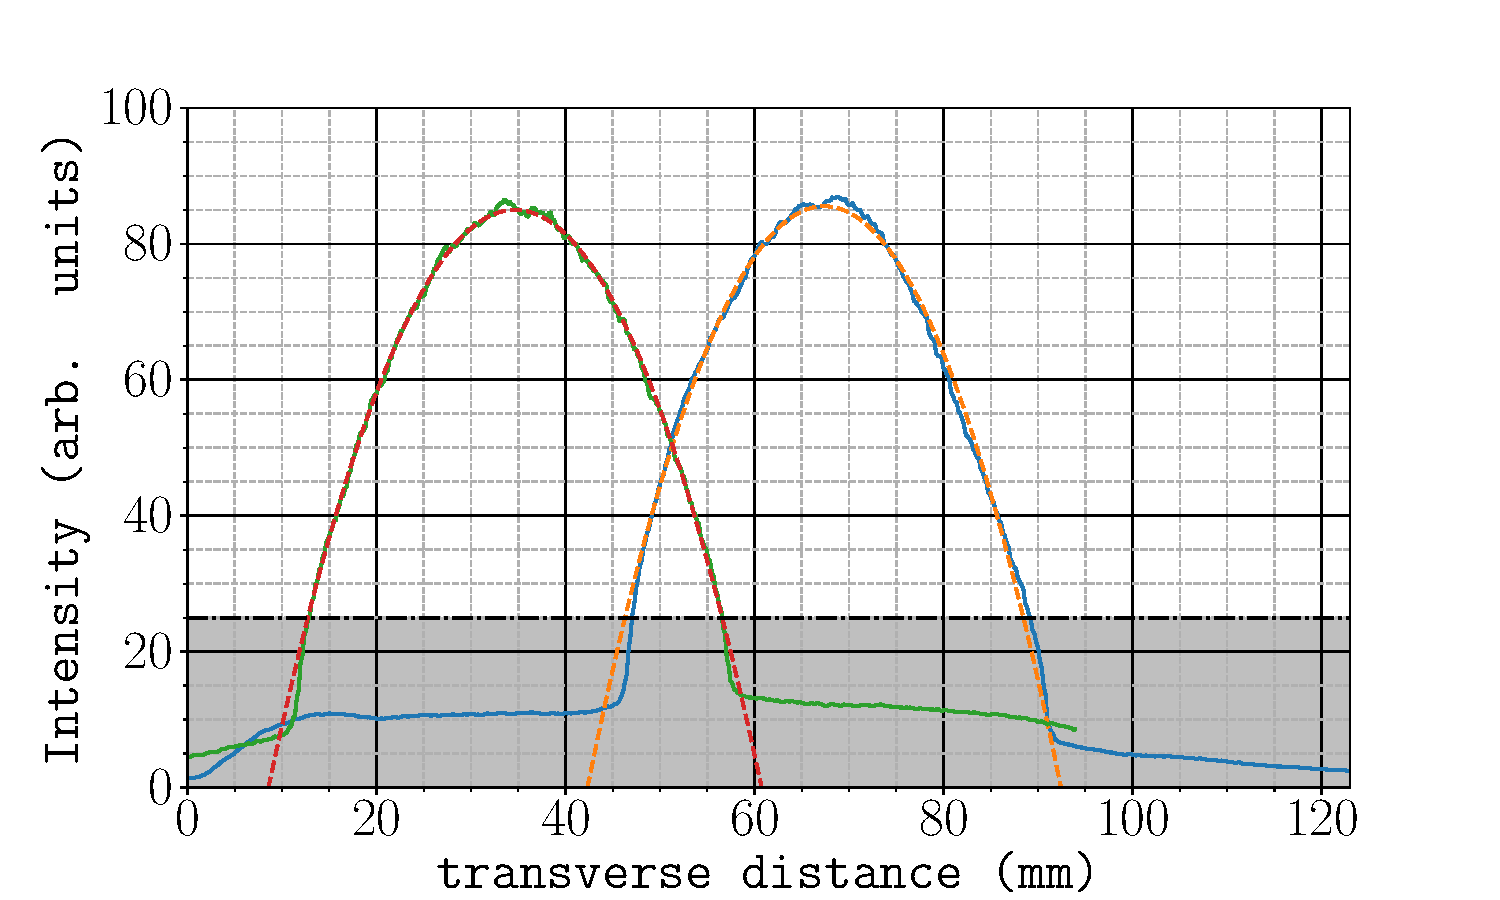
\includegraphics{beam_examp}}\label{fig:beam_examp}}
	\subfloat[][]{\scalebox{0.3}{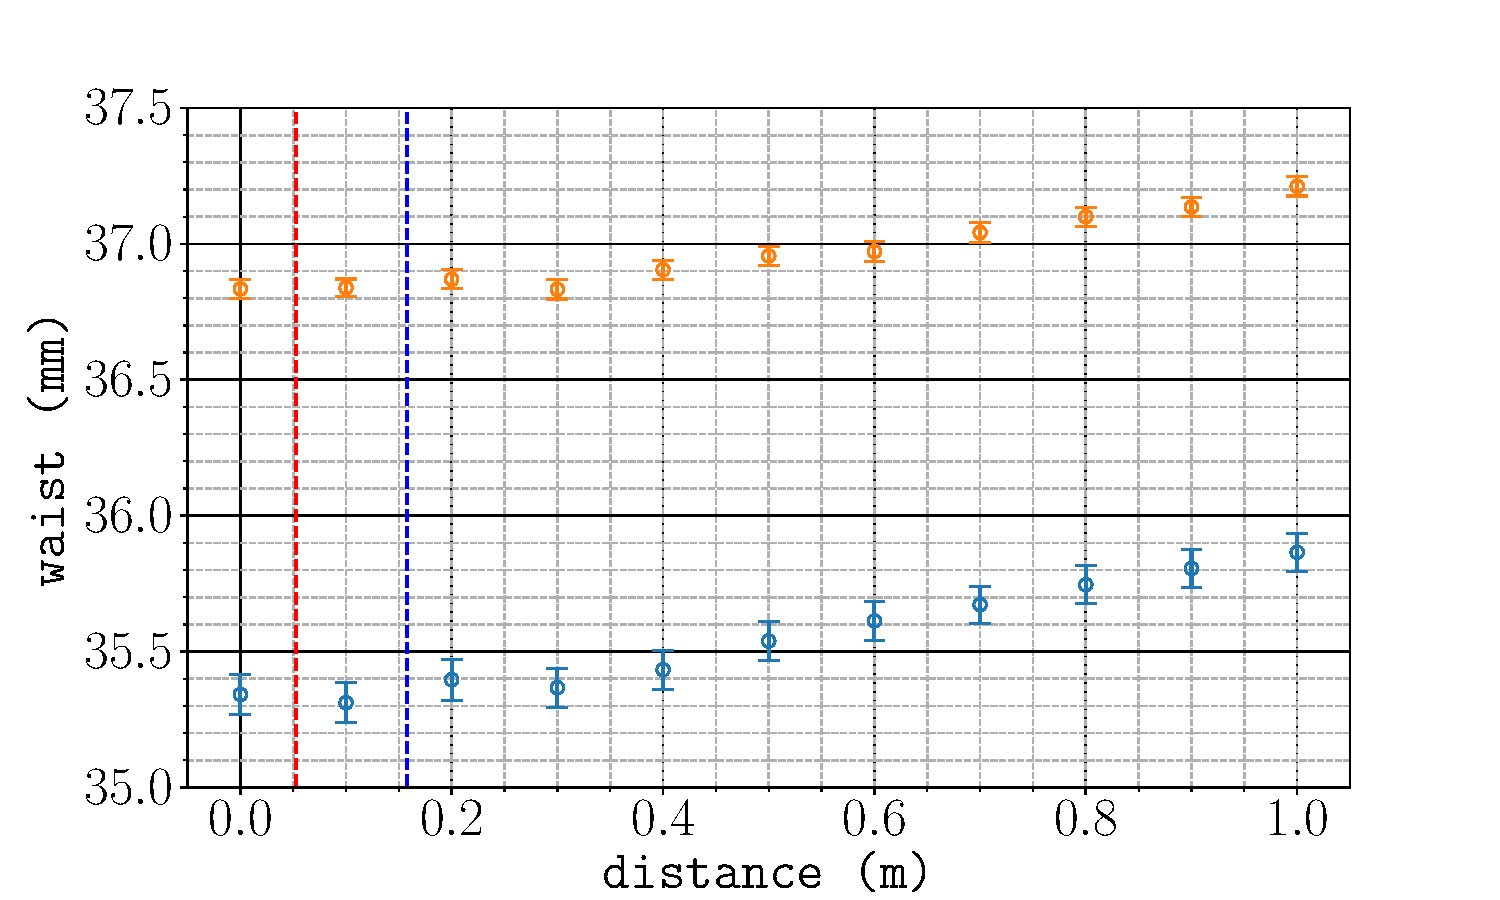
\includegraphics{beam_waist}}\label{fig:beam_waist}}
	\caption[Measured Raman beam waist]{Raman beam waist measured over a distance
		of \sivalue{1}{\metre}, shown in \textbf{(a)}. The waist along the
		horizontal and vertical axes are indicated in blue and orange respectively.
		The dashed lines indicate the approximate propagation distance of each beam
		at the position of the atoms. \textbf{(b)} shows the intensity profile along
		each axis, with the fitted parabola. The dot-dashed line is a threshold
		intensity value, which excludes pixels from outside the spatial extent of
		the beam.} 
  \label{fig:beam_waist_plots} 
\end{figure}
\section{Retro-Reflection Assembly}\label{subsec:setup_ramanmirror} The
		Raman transitions used in the interferometer need to be driven by
		counter-propagating light fields to give a large momentum transfer of \(2
		\hbar k\) to the atoms. The two beams enter from the same fibre
    input, with polarisations $\sigma^+$ and $\sigma^-$, and a
		mirror is used to retro-reflect them. The retro-reflection assembly includes
		a \ac{qwp} to reverse the circular polarisation of each light
    beam. The polarisation then ensures that the Raman transition is
    driven by counter-propagating beams - either $\sigma^+ - \sigma^+$
    or $\sigma^- - \sigma^-$. This retro-reflection part of the
    optical
    is the most crucial for avoiding transverse spatial variation in
    the Raman phase.\par\noindent
		The mirror is also manufactured by Light Machinery, and the \ac{qwp} is made
		to the same specifications as the one that circularly polarises the incoming
		beams.  During the manufacturing process, the waveplates and mirror were
		polished to reduce irregularities in the thickness of each \ac{qwp} and the
		surface of the mirror. \FigureRef{fig:waveplate_map} shows the variation in
		the thickness of the waveplate in front of the triplet lens, measured by
		Light Machinery using a white light interferometer. This has a standard
		deviation of \sivalue{4.62}{\nano\metre} and corresponds a standard
		deviation of the optical path length of \pow{8.6}{-3}\(\lambda\).
\begin{figure}[!htbp] 
  \centering
  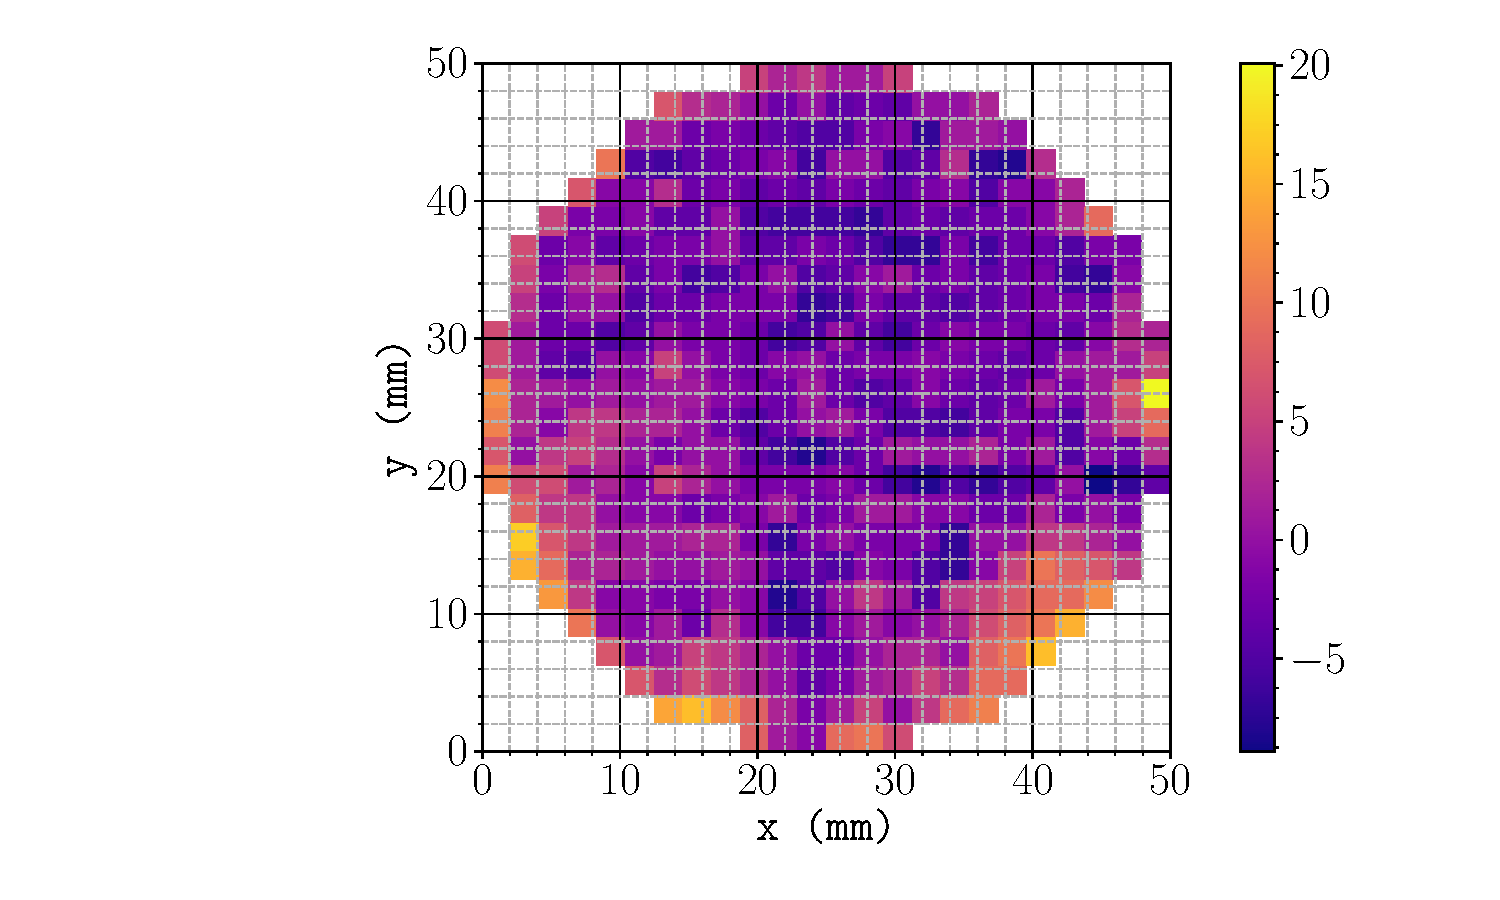
\includegraphics[width=0.7\textwidth]{waveplate.pdf}
  \caption[Quarter-wave plate thickness variation.]{Thickness of the first \ac{qwp}, measured by a white light
		interferometer. The value is given in \sivalue{}{\nano\metre} as a
		difference from the mean thickness. The standard deviation of this thickness
		is \sivalue{4.62}{\nano\metre} and a peak-to-valley (PV) of {\textbf need
		number here}. Equivalent surface data for the other \ac{qwp} and mirror were
		not provided by Light Machinery, but had a PV thickness variation of
		\sivalue{19}{\nano\metre} and
		\sivalue{9}{\nano\metre} respectively.} \label{fig:waveplate_map}
\end{figure} 
The \ac{qwp} and mirror are fixed onto the front
plate of a UHV compatible MDI-HS mirror mount, manufactured by Radiant dye. The
horizontal and vertical tilts of the mirror can be adjusted using two thumbscrew
actuators which cause the front plate to tip. This mount
is designed for high stability, but of course the alignment will still drift
over time. To avoid the need to periodically open the chamber to realign the
mirror, a piezo-electric stack is placed between each actuator and the front
plate so that the tilt of the mirror can be adjusted externally. Each
piezo-stack is connected to a high-voltage feedthrough, so that their length
(and hence mirror tilt) can be finely adjusted by controlling the voltage
applied across them. A control voltage ranging between 0--\sivalue{10}{\volt} is
amplified by a controller to give an applied voltage across the piezo stack
between -10--\sivalue{150}{\volt}. This corresponds to a travel range of
\subsection{In-Situ Alignment and Optimisation}\label{sec:in_situ} 
After mounting the Raman optical system inside the chamber, the
mirror had to be aligned to retro-reflect the light. When the mirror is close to
perpendicular to the light's wavevector, some of the power in the reflected beam
couples back into the fibre. In principle, this power is maximised when the
mirror is exactly perpendicular so maximising this power is a useful technique
to align the mirror. A 99:1 fibre splitter was used to couple light into the
chamber, which provided a means to measure the back-reflected power without
needing any free-space optics. This was set up so that 99\% of the incoming
light entered the chamber, with the other 1\% coupled into the corresponding
output port. The beam-splitter acts reversibly so 1\% of the
back-reflected light which couples into vacuum fibre exits the fibre-splitter on
the other input port.  
By splitting off only a small amount of
power, most of the light enters the chamber and is thus useful for
driving Raman transitions. The back-reflected power can be used to 
continuously monitor the alignment of the mirror.
%However, it was found that this fibre
%splitter did not sufficiently preserve the polarisation of the
%incoming light. A drift of the polarisation from its output rendered
%this continuous monitoring impractical. 
\par\noindent 
Out sponsors, the dstl, want the accelerometer to have an automated
start-up procedure, so an automatic routine was devised to do align
the retro-reflector. This was carried out using
a pair of bipolar stepper motors to adjust each thumbscrew. The revolution of these motors was controlled using
an Arduino microcontroller, which communicated with the computer using a serial
interface.  The motors rotated by 0.9\(\deg\)/step, which corresponds to a tilt
of the mirror by \sivalue{18.1}{\micro\radian}. 
\par\noindent 
Using this method, the mirror mount was aligned so
that the maximum of the back-reflected power was reachable with the piezo
stacks. Of course, it was foreseeable that the mirror would need to be
periodically realigned, which would require another systematic iteration through
the voltages applied to each piezo stack. Given that this search was quite time
consuming, it was not a practical way to maintain alignment. To improve upon
this, an optimisation method using the Nelder-Mead simplex
algorithm~\cite{Nelder1965} was implemented. This method is suitable for
optimising multidimensional functions and has been used to demonstrate the
automatic alignment of a fibre with up to 6 degrees of freedom~\cite{Zhang2004}.
\par\noindent
The Nelder-Mead algorithm aims to optimise the value of an objective
function (in this instance, the optical power measured as a voltage by a
photodiode) by sampling the function at various locations. For \(n\) parameters,
a set of \(n-1\) points distributed randomly across the parameter space are
chosen as the initial simplex. These are sorted in decreasing order of the value
of the objective function and the algorithm proceeds by performing geometric
transformations on this simplex, by sequentially reflecting, expanding and
contracting it. Each step starts with a reflection about the line
between the two greatest values. The coordinates of the simplex are updated if
the function has a greater value at the location given by one of these
transformations, until the algorithm converges on a maximum value. As with many
optimisation algorithms, the Nelder-Mead method has the potential to converge on
a local optimum, but this is alleviated by expanding the simplex to look for
more optimal values. The termination of the algorithm was decided by using the
standard deviation of the last 5 values. Empirically, it was found that
terminating when the standard deviation was less than \sivalue{10}{\micro\volt}
resulted in stable performance of the algorithm, even when the signal-to-noise
ratio of the measured voltage was poor. An example of this algorithm aligning
the mirror mount is presented in \FigureRef{fig:simplex_optimisation}. To verify
that the converged value was optimal, a systematic scan of the piezo stack
control voltages in the region around this value was also carried out. In this
case, the algorithm converged on a local maximum, that was very close
to the global maximum and greatly enhanced
the coupling efficiency of the reflected light back into the fibre. The
difference in the piezo control voltages between the local and global
maxima corresponded 
to a tilt of the mirror mount of less
than \sivalue{13}{\micro\radian}. This scheme was thus selected as the
one to incorporate into the start-up routine for the accelerometer.
\begin{figure}[!htbp] 
  \centering
	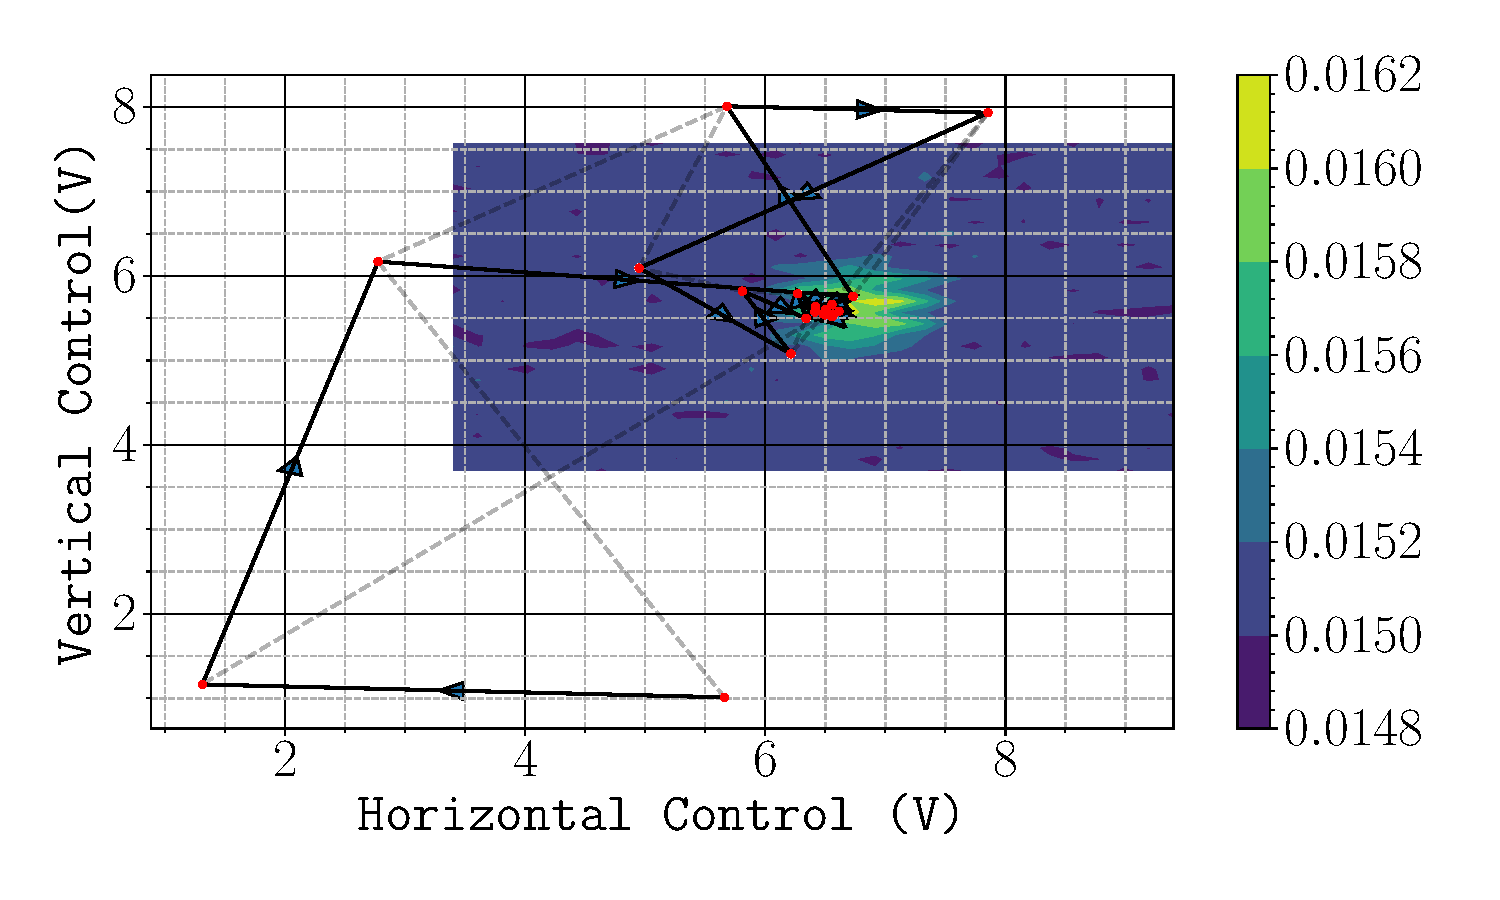
\includegraphics[width=0.7\textwidth]{simplex_alignment}
	\caption[Automatic mirror alignment using the Nelder-Mead simplex
		algorithm.]{Automatic mirror alignment using the Nelder-Mead simplex
		algorithm. A sequence of geometric transformations on the initial
    simplex are used to converge on the optimum point, where the
    back-reflected power is maximised. The shaded lines indicate the simplex bounded by
    the three co-ordinates at each iteration.
		A raster scan of the piezo control
		voltages close to the optimum is also plotted. The irregular shape of the
		measured power is a result of a hysteresis effect when the horizontal
		control voltage was changed from its maximum value to the minimum.}
		\label{fig:simplex_optimisation} 
  \end{figure}
\subsection{The Mechanical Accelerometer}\label{subsec:raman_mems}
The interferometer phase is proportional to the acceleration of the
retro-reflecting mirror relative to the freely-falling atoms. However,
the sinusoidal interferometer signal is periodic with period
\(\Delta a = \frac{\pi}{\keff T^2}\), so we need to know the order
number of the fringe before the acceleration can be deduced from the
signal. For this reason, a mechanical (MEMS)
accelerometer is mounted on the back of the retro-reflecting mirror to determine the acceleration up to the fringe spacing and the interferometer measures the acceleration more
precisely. 
%The accelerometer is also sensitive to vibrations of the
%retro-reflecting mirror, so it can be used to filter the effects of vibration
%noise on the interferometer signal.  
The MEMS accelerometer is also sensitive to vibrations of the
retro-reflecting mirror and can be used to characterise the
vibration-induced phase noise. This is discussed in more detail
in~\SectionRef{subsec:vibration_sensitivity}. This technique enables
accurate measurements of acceleration in high-noise environments and has been
used to measure the acceleration due to gravity at the centre of
Paris~\cite{Merlet2009} and in parabolic aircraft
flights~\cite{Geiger2011a,Barrett2016}. 
\par\noindent 
The accelerometer is a navigation-grade AI-Q-2010 manufactured by \textit{Innalabs}. This particular
device was chosen for its low noise specification of
<\sivalue{7}{\micro\g} in the 0-\sivalue{100}{\Hz} bandwidth. For a pulse separation \(T
= \sivalue{25}{\milli\second}\), the fringe spacing is
\(\sivalue{31.2}{\micro\g}\) so it is sensitive enough to measure the
acceleration to within one fringe. A schematic of this device is shown
in~\FigureRef{fig:innalabs}. It operates using a quartz pendulum which is is
free to move about one
axis~\cite{Foote1992,Lawrence1998}\nocite{Lawrence1998a}. Under an acceleration, the
deflection of the pendulum is capacitively detected. A servo loop circuit drives
a current through the coils to restore the position of the pendulum. This
current is directly proportional to the acceleration of the pendulum. This model
has a nominal scale factor of \sivalue{1.235976}{\milli\ampere\per\g}. The
acceleration is measured using a load resistance of \sivalue{6}{\kilo\ohm} to
give an output voltage of \sivalue{7.56}{\volt\per\g}.
\begin{figure}[!htbp] \centering
	\resizebox{0.5\textwidth}{!}{\input{innalabs.pdf_tex}}
	\caption[Innalabs accelerometer cross-section]{Cross-section of the Innalabs
		AI-Q-2010 accelerometer.} \label{fig:innalabs}
\end{figure}

\section{Conclusion}
This chapter has motivated the need for low wavefront distortions to achieve sensitive measurements of acceleration, particularly when there is significant transverse motion across the Raman beam. Following this, the in-vacuum optical system was introduced. This helps to reduce the effect of wavefront distortions by not transmitting the beam through an optical viewport. Finally, the retro-reflection assembly used to produce the counter-propagating beams has been presented.  
